\section{Experiments}
\subsection{Experimental Set-up}
% 0.5-1 page
% \begin{itemize}
%     \item Algorithms we are evaluating
%     \begin{itemize}
%         \item MPDA, WPDA
%         \item Probabilistic-based that always selects the best stable matching with a probability
%         \item Probabilistic-based that always selects the best matching with a probability
%         \item [Stretch] Deterministic algorithm that always selects the best sw with a consistency above a certain threshold
%     \end{itemize}
%     \item Dynamics
%     \item Number of agents, time steps, etc.
%     \item Evaluation set-up
% \end{itemize}
\paragraph{Dynamics Setting} For each agent, we independently initialize each utility value by sampling from a normal distribution $\mathcal{N}(\mu_1, \sigma_1^2)$ with scalar mean $\mu_1 \in \mathbb{R}$ and variance $\sigma_1^2 \in \mathbb{R}$. We further normalize the utilities such that each agent's utility vector has a total sum of 1. In addition, we set each agent's excitement values by again independently sampling from a normal distribution $\mathcal{N}(\mu_2, \sigma_2^2)$. We clip each excitement value at 0 to ensure that the excitement is non-negative.

\paragraph{Algorithms} We implement both the Men Proposing Deferred Acceptance (MPDA) and the Women Proposing Deferred Acceptance (WPDA) algorithms, which are guaranteed to return a stable matching. In addition, we implement a family of deterministic algorithms (Det) and a family of probabilistic algorithms (Prob), described as follows.

Det: This is a family of algorithms parameterized by $c \in [0, 1]$ and returns a perfect matching satisfying $$M^{t+1} = \argmax_{\mbox{consistency}(M^t, M) \ge c}{\mbox{sw}(M)}.$$ In other words, the generated matching $M^{t+1}$ is the matching maximizing the social welfare subjected to the condition that the consistency is at least $c$ compared to the most recent match. For computational efficiency, instead of enumerating through all possible matching that has at least consistency $c$, we approximate by fixing $N * c$ couples in $M^t$ that have the highest social welfare according to the updated utilities $\overrightarrow{u}^{t+1}, \overrightarrow{v}^{t+1}$, and then perform the Hungarian Algorithm~\cite{Kuhn55thehungarian,Kuhn56thehungarian,Munkres1957Assignment} over the remaining men and women to obtain the maximum weight perfect bipartite matching, with the weight between a man node $m_i$ and a woman node $w_j$ being $u_i^{t+1}(w_j) + v_j^{t+1}(m_i)$. As a result, the generated new matching has at least consistency $c$ and a reasonably large social welfare.



\subsection{Results}
0.5 - 1 page
Figures and analysis
\begin{itemize}
    \item Evaluation of the algorithms (trade-off plot)
    \begin{itemize}
        \item scatter plot for the algorithm family
        \item variance plot for the algorithm family
    \end{itemize}
    \item Evaluation with various dynamics
    \begin{itemize}
        \item Plot the trade off curve with MPDA and update with match
    \end{itemize}
\end{itemize}

\begin{figure}
    \centering
        \begin{subfigure}[b]{0.49\textwidth}
         \centering
         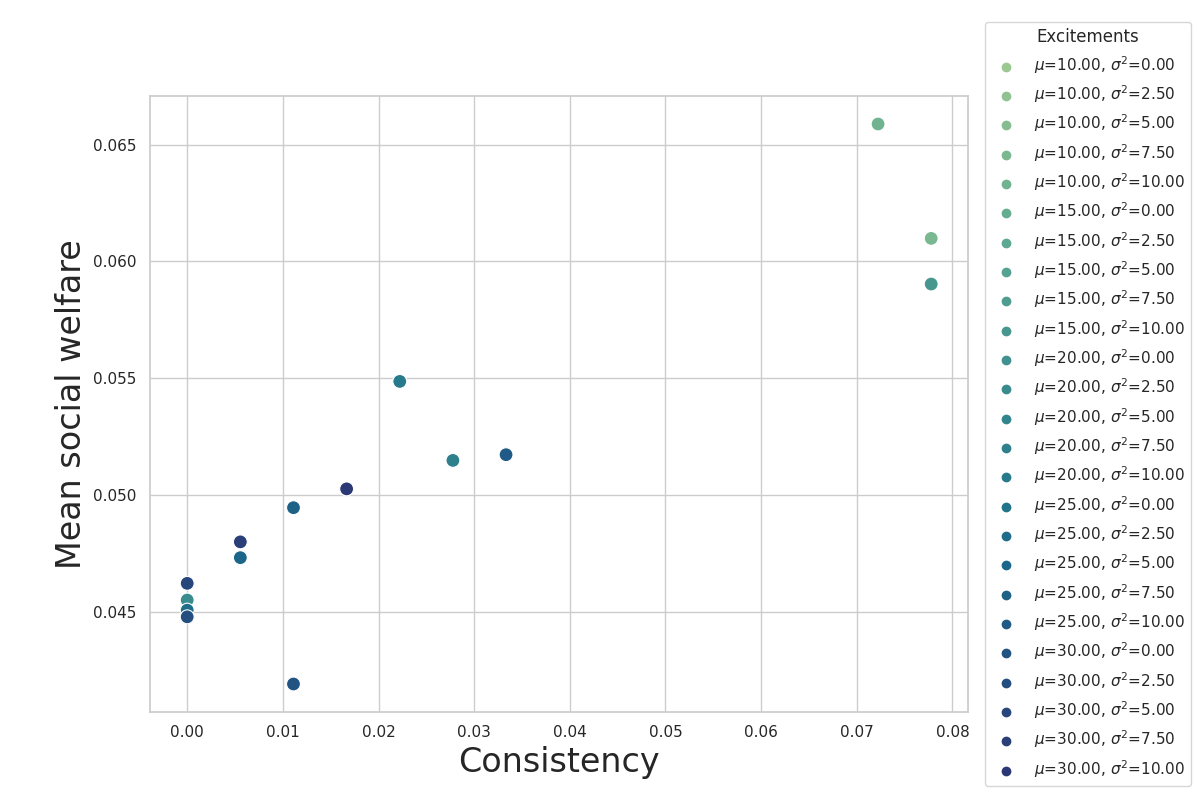
\includegraphics[width=\textwidth]{figures/mpda_dynamics_initliazation.png}
         \caption{Dynamic Initialization}
         \label{fig:init}
        \end{subfigure}
         \begin{subfigure}[b]{0.49\textwidth}
         \centering
         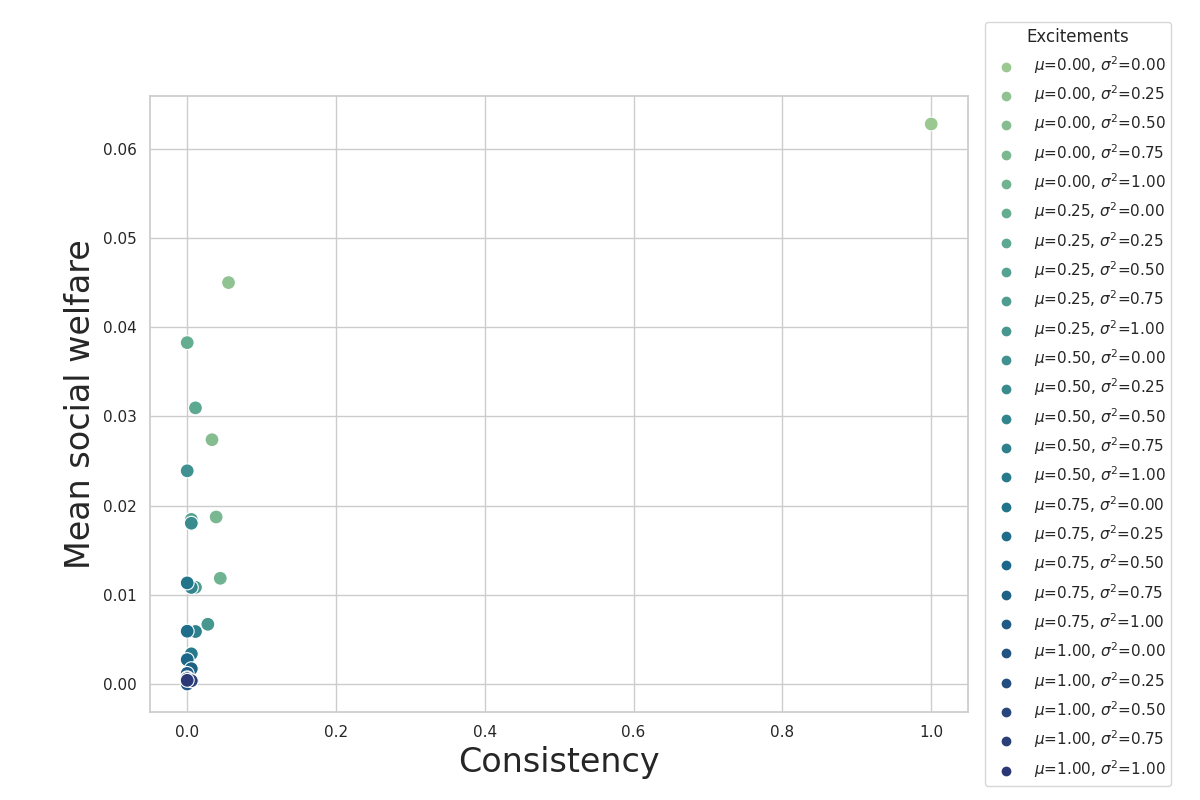
\includegraphics[width=\textwidth]{figures/mpda_dynamics_excitement.png}
         \caption{Dynamic Excitement}
         \label{fig:excite}
     \end{subfigure}
    \caption{Mean social welfare vs. consistency for MPDA applied to two dyanmic scenarios; (a) fixed excitement ($\mu=0.5, \sigma^2=0.5$) with  varying initialization ($\mu \in [10, 20], \sigma^2 \in [0, 10]$); (b) fixed initialization ($\mu=20, \sigma^2=5$) with varying excitement ($\mu \in [0, 1], \sigma^2 \in [0, 1]$).}
    \label{fig:mpda_dynamics}
\end{figure}